% Options for packages loaded elsewhere
\PassOptionsToPackage{unicode}{hyperref}
\PassOptionsToPackage{hyphens}{url}
%
\documentclass[
]{article}
\usepackage{lmodern}
\usepackage{amssymb,amsmath}
\usepackage{ifxetex,ifluatex}
\ifnum 0\ifxetex 1\fi\ifluatex 1\fi=0 % if pdftex
  \usepackage[T1]{fontenc}
  \usepackage[utf8]{inputenc}
  \usepackage{textcomp} % provide euro and other symbols
\else % if luatex or xetex
  \usepackage{unicode-math}
  \defaultfontfeatures{Scale=MatchLowercase}
  \defaultfontfeatures[\rmfamily]{Ligatures=TeX,Scale=1}
\fi
% Use upquote if available, for straight quotes in verbatim environments
\IfFileExists{upquote.sty}{\usepackage{upquote}}{}
\IfFileExists{microtype.sty}{% use microtype if available
  \usepackage[]{microtype}
  \UseMicrotypeSet[protrusion]{basicmath} % disable protrusion for tt fonts
}{}
\makeatletter
\@ifundefined{KOMAClassName}{% if non-KOMA class
  \IfFileExists{parskip.sty}{%
    \usepackage{parskip}
  }{% else
    \setlength{\parindent}{0pt}
    \setlength{\parskip}{6pt plus 2pt minus 1pt}}
}{% if KOMA class
  \KOMAoptions{parskip=half}}
\makeatother
\usepackage{xcolor}
\IfFileExists{xurl.sty}{\usepackage{xurl}}{} % add URL line breaks if available
\IfFileExists{bookmark.sty}{\usepackage{bookmark}}{\usepackage{hyperref}}
\hypersetup{
  pdftitle={COVID-19 condition study in the United States},
  hidelinks,
  pdfcreator={LaTeX via pandoc}}
\urlstyle{same} % disable monospaced font for URLs
\usepackage[margin=1in]{geometry}
\usepackage{longtable,booktabs}
% Correct order of tables after \paragraph or \subparagraph
\usepackage{etoolbox}
\makeatletter
\patchcmd\longtable{\par}{\if@noskipsec\mbox{}\fi\par}{}{}
\makeatother
% Allow footnotes in longtable head/foot
\IfFileExists{footnotehyper.sty}{\usepackage{footnotehyper}}{\usepackage{footnote}}
\makesavenoteenv{longtable}
\usepackage{graphicx,grffile}
\makeatletter
\def\maxwidth{\ifdim\Gin@nat@width>\linewidth\linewidth\else\Gin@nat@width\fi}
\def\maxheight{\ifdim\Gin@nat@height>\textheight\textheight\else\Gin@nat@height\fi}
\makeatother
% Scale images if necessary, so that they will not overflow the page
% margins by default, and it is still possible to overwrite the defaults
% using explicit options in \includegraphics[width, height, ...]{}
\setkeys{Gin}{width=\maxwidth,height=\maxheight,keepaspectratio}
% Set default figure placement to htbp
\makeatletter
\def\fps@figure{htbp}
\makeatother
\setlength{\emergencystretch}{3em} % prevent overfull lines
\providecommand{\tightlist}{%
  \setlength{\itemsep}{0pt}\setlength{\parskip}{0pt}}
\setcounter{secnumdepth}{-\maxdimen} % remove section numbering

\title{COVID-19 condition study in the United States}
\author{}
\date{\vspace{-2.5em}}

\begin{document}
\maketitle

{
\setcounter{tocdepth}{3}
\tableofcontents
}
\#\texttt{\{r,\ echo=FALSE\}\ \#Sys.setenv("plotly\_username"="lysethan")\ \#Sys.setenv("plotly\_api\_key"="2xTbFH705WoS1d0k6UEg")\ \#}

\hypertarget{introduction}{%
\subsection{Introduction}\label{introduction}}

COVID-19 is a global pandemic that affects our health and life. By
exploring the COVID-19 condition, we can make take possible actions to
better contain its spread and make plans for the future. In this
project, we mainly study the COVID-19 condition in the United States.

How is the COVID-19 condition in the United States now? The question can
be answered from the following perspectives:

\begin{itemize}
\tightlist
\item
  Q1: Condition Overview: latest numbers about the tests, confirmed
  cases, deaths and recoveries.
\item
  Q2: Pandemic Tendency: the tendency of COVID-19 infection in terms of
  new tests, new positives and new deaths.
\item
  Q3: Community Infection Status: the infection status of different
  race/ethnicity and age groups.
\item
  Q4: Population Infection Rate: the population infection rate in
  different states, which can be a indicator of virus spreading level.
\item
  Q5: Key Information: the key latest information or notes we should pay
  attention to.
\end{itemize}

\hypertarget{methods}{%
\subsection{Methods}\label{methods}}

The data for this study comes from three sources:

\begin{enumerate}
\def\labelenumi{\arabic{enumi}.}
\tightlist
\item
  \url{https://covidtracking.com/data/api}
\item
  \url{https://covid.cdc.gov/covid-data-tracker/\#demographics}
\item
  \url{https://github.com/nytimes/covid-19-data}
\end{enumerate}

The data are details are described as follows:

\begin{itemize}
\tightlist
\item
  cases\_by\_age\_group.csv \# COVID-19 cases in United States grouped
  by age bins, last updated at Nov 17 2020 12:18PM.
\item
  cases\_by\_race\_ethnicity\_\_all\_age\_groups.csv \# COVID-19 cases
  in United States grouped by races/ethnicities, last updated at Nov 17
  2020 12:18PM.
\item
  daily.csv \# historical COVID-19 of the United States, daily recorded
\item
  deaths\_by\_age\_group.csv \# COVID-19 deaths in United States grouped
  by age bins, last updated at Nov 17 2020 12:18PM.
\item
  deaths\_by\_race\_ethnicity\_\_all\_age\_groups.csv \# COVID-19 deaths
  in United States grouped by races/ethnicities, last updated at Nov 17
  2020 12:18PM.
\item
  states\_current.csv \# The most recent COVID data for every state.
\item
  states\_daily.csv \# all COVID data available for every state since
  tracking started.
\item
  states\_info.csv \# Basic information about states, including notes
  about the data.
\item
  us\_census\_2018\_population\_estimates\_states.csv \# population data
  of each states
\end{itemize}

This project uses the following packages to achieve the analysis:

\begin{longtable}[]{@{}ll@{}}
\toprule
packages & functions\tabularnewline
\midrule
\endhead
data.table & data readin\tabularnewline
tidyverse & data wrangling\tabularnewline
dplyr & data transforming\tabularnewline
plotly & generate interactive graphics\tabularnewline
DT & render R data frames to tables\tabularnewline
knitr & render rmarkdown files to htmls, pdfs, etc.\tabularnewline
stringr & handle strings in R\tabularnewline
sjPlot & render data frames to publish-style tables\tabularnewline
ggthemes & themes for ggplot graphics\tabularnewline
scales & tool for graphics scaling\tabularnewline
ggwordcloud & generate word cloud\tabularnewline
ggpubr & arrange ggplot objects\tabularnewline
\bottomrule
\end{longtable}

\hypertarget{results}{%
\subsection{Results}\label{results}}

\hypertarget{q1-condition-overview}{%
\subsubsection{Q1: Condition Overview}\label{q1-condition-overview}}

Here is the summary of the latest numbers about the total tests,
accumulated confirmed case numbers, accumulated deaths, accumulated
recoveries.

\begin{longtable}[]{@{}rrrrr@{}}
\toprule
\begin{minipage}[b]{0.08\columnwidth}\raggedleft
date\strut
\end{minipage} & \begin{minipage}[b]{0.11\columnwidth}\raggedleft
total tests\strut
\end{minipage} & \begin{minipage}[b]{0.31\columnwidth}\raggedleft
accumulated confirmed case numbers\strut
\end{minipage} & \begin{minipage}[b]{0.20\columnwidth}\raggedleft
accumulated recoveries\strut
\end{minipage} & \begin{minipage}[b]{0.17\columnwidth}\raggedleft
accumulated deaths\strut
\end{minipage}\tabularnewline
\midrule
\endhead
\begin{minipage}[t]{0.08\columnwidth}\raggedleft
20201117\strut
\end{minipage} & \begin{minipage}[t]{0.11\columnwidth}\raggedleft
170315721\strut
\end{minipage} & \begin{minipage}[t]{0.31\columnwidth}\raggedleft
11202899\strut
\end{minipage} & \begin{minipage}[t]{0.20\columnwidth}\raggedleft
4293640\strut
\end{minipage} & \begin{minipage}[t]{0.17\columnwidth}\raggedleft
239784\strut
\end{minipage}\tabularnewline
\bottomrule
\end{longtable}

\hypertarget{q2-pandemic-tendency}{%
\subsubsection{Q2: Pandemic Tendency}\label{q2-pandemic-tendency}}

The tendency of COVID-19 can reflect how will this pandemic will proceed
into the future. Is it getting better or worse? We can illustrate the
pandemic tendency using three important variables: New COVID-19 Tests,
New Positive Cases, New Death Cases. The result is shown in the
following graph.

\begin{center}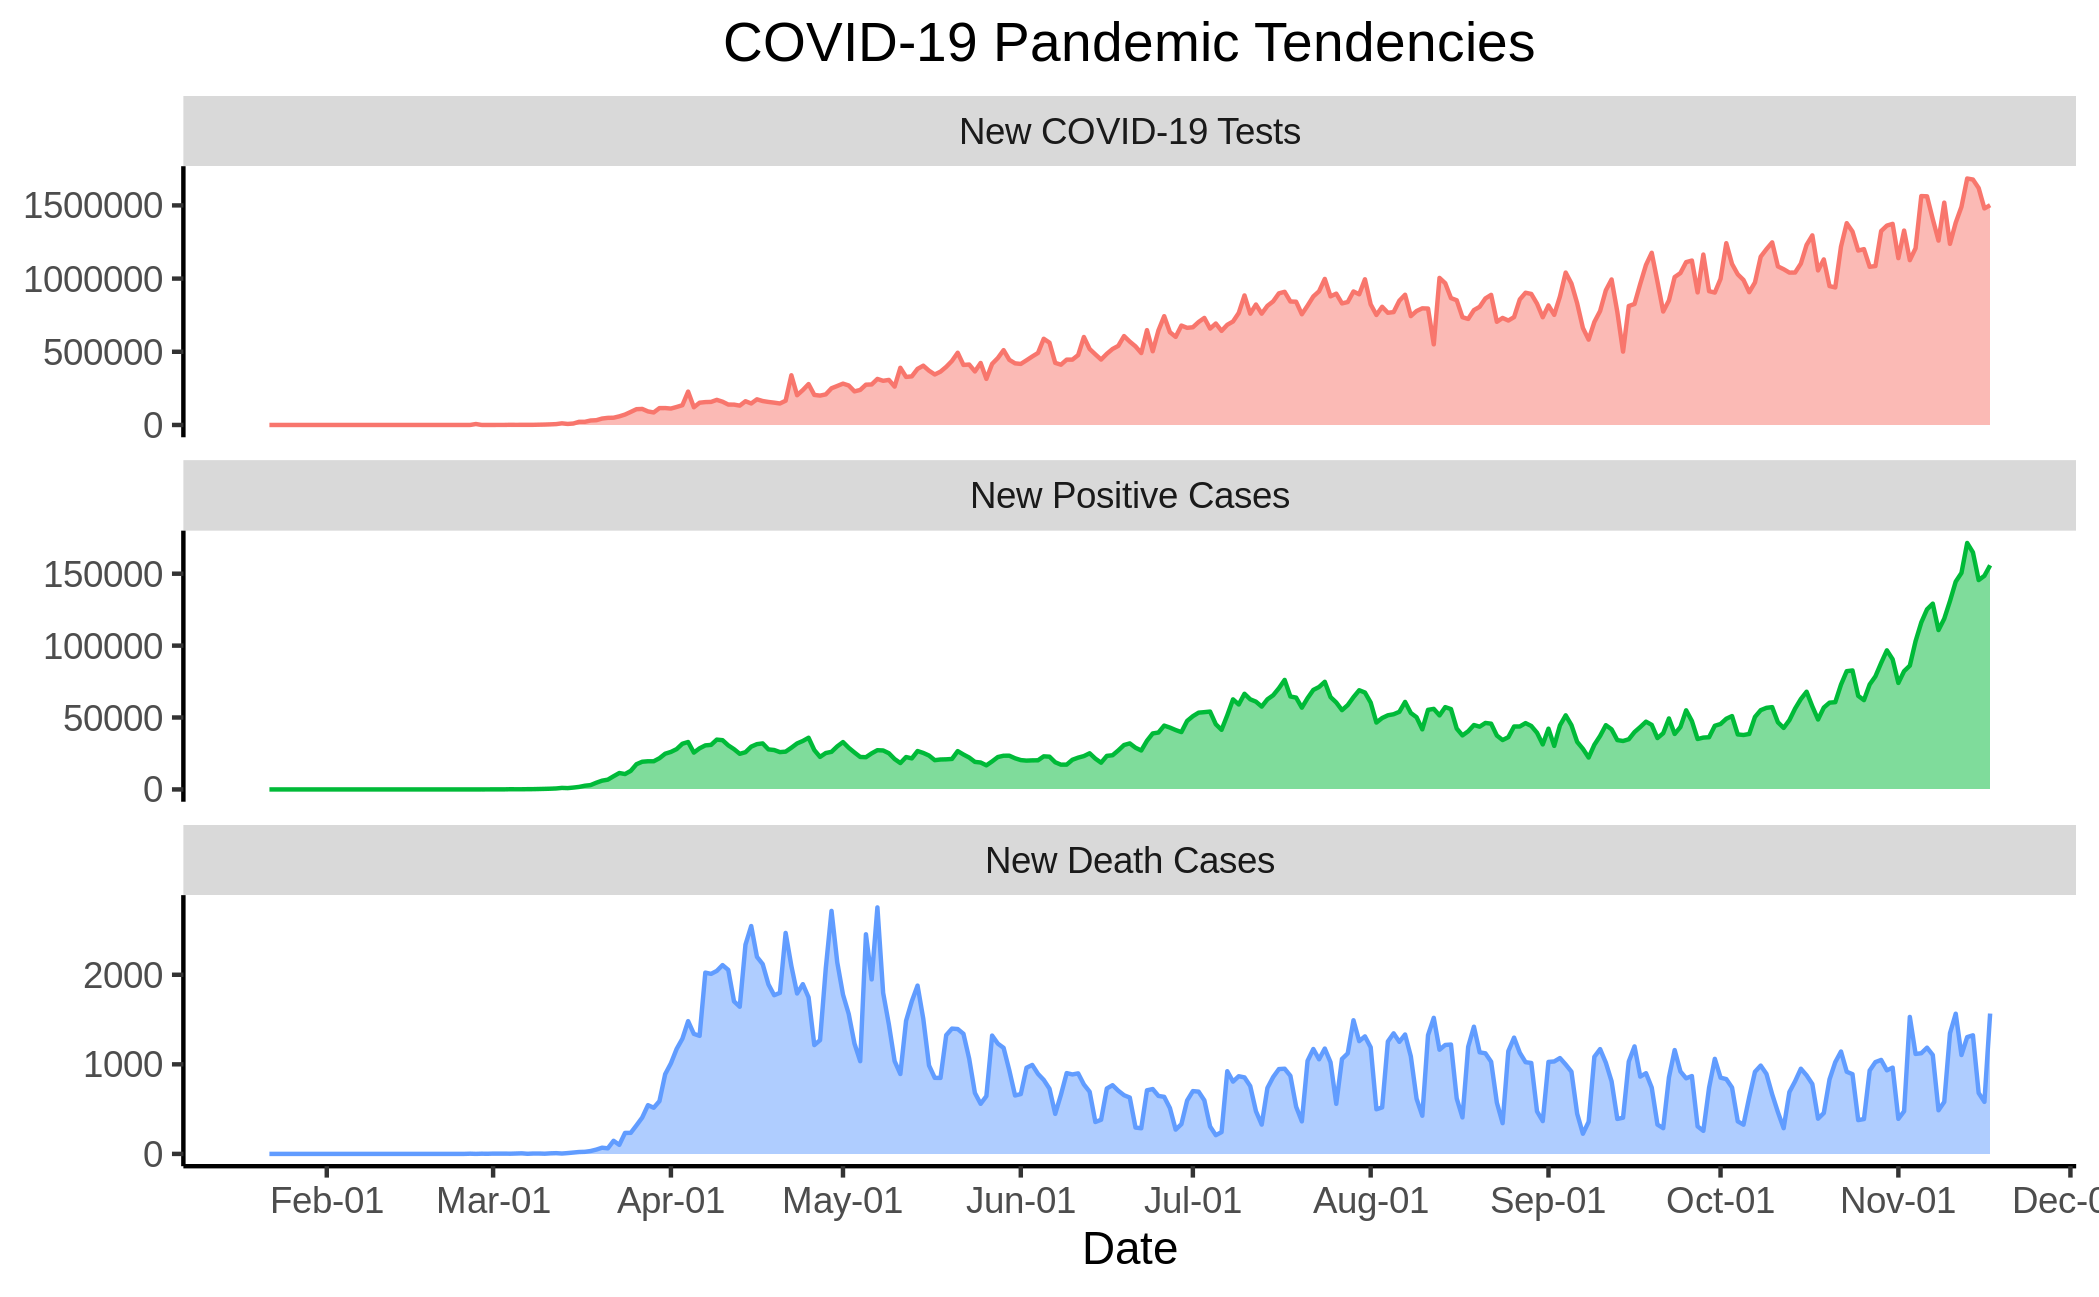
\includegraphics[width=1\linewidth]{tendency} \end{center}

We can see that we are doing more and more COVID-19 testing. And the
line graph of new positive cases depicts the tendency of the COVID-19
pandemic. It shows there are more and more people getting infected with
COVID-19. The curve indicates that the virus spreading is speeding up as
the time goes. Therefore, we have not reached the turning point in which
the actual condition gets better.

From the curve of the New death cases, we can see the new death cases is
becoming flat and not increasing like new confirmed cases, plausibly
indicating that COVID-19 virus is less harmful than before or we are
more experienced to cure the disease. However, this may subject to many
factors' influences.

\hypertarget{q3-community-infection-status}{%
\subsubsection{Q3: Community Infection
Status}\label{q3-community-infection-status}}

Different age groups may have different susceptibility towards the virus
due to their different immune levels. In addition, the virus infection
may also differs with respect to races and ethnicities. We gathered the
data from \url{https://covid.cdc.gov} to discover the infection status
of different age groups or races and ethnicities.

\begin{center}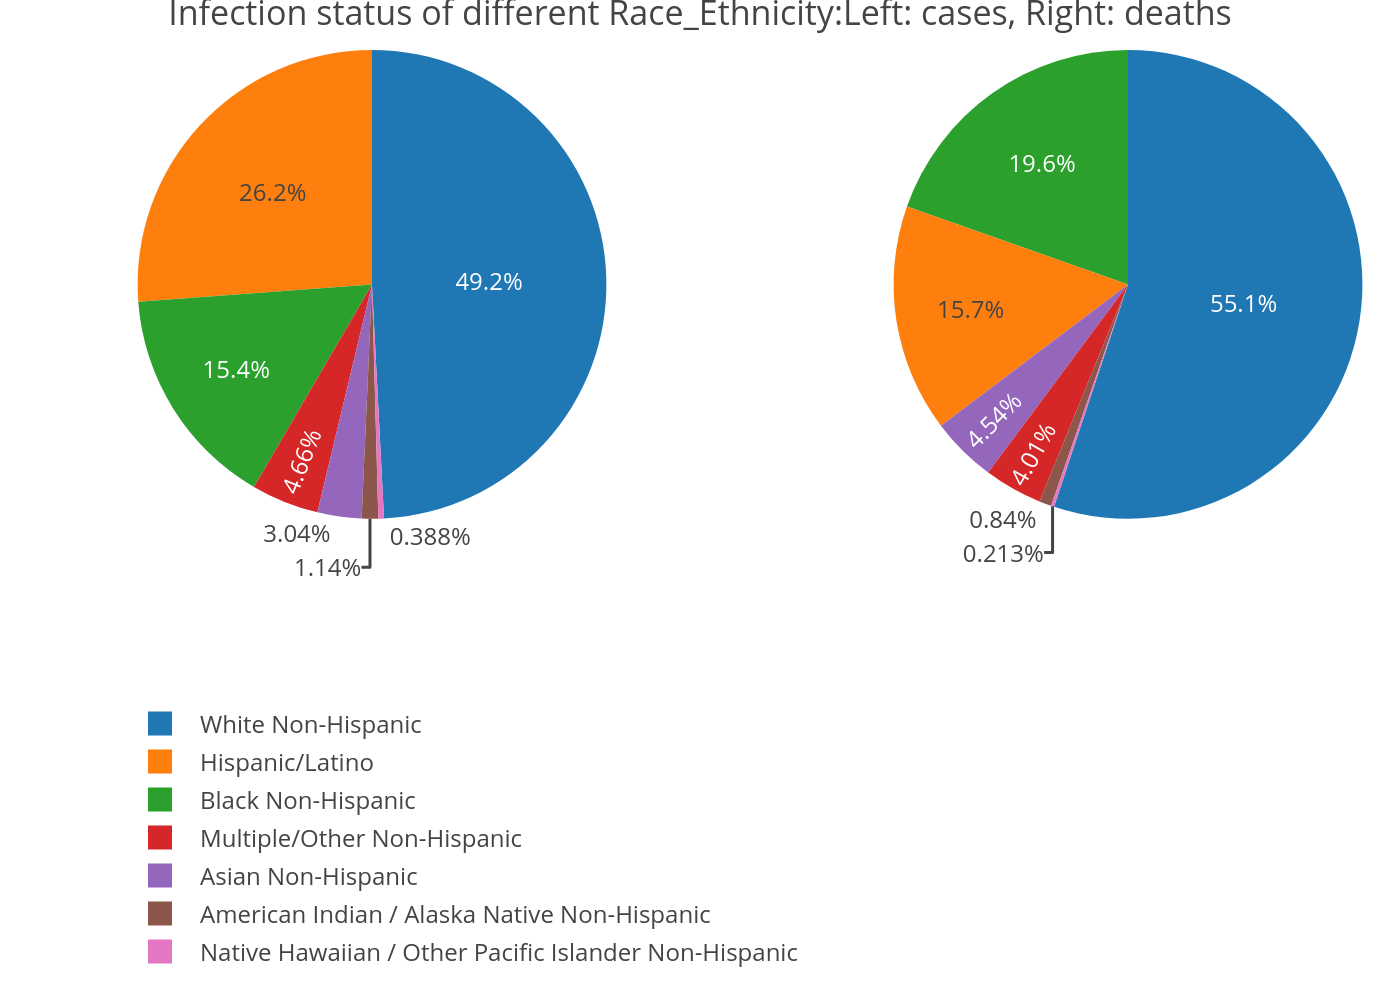
\includegraphics[width=1\linewidth]{race} \end{center}

From the graph, we can find that the differences among races and
ethnicities are large. White Non-Hispanic has both the highest infection
rate and covid-death rate, whereas Asian Non-Hispanic, American Indian,
Native Hawaiian has significantly low infection rate and death rate.

\begin{center}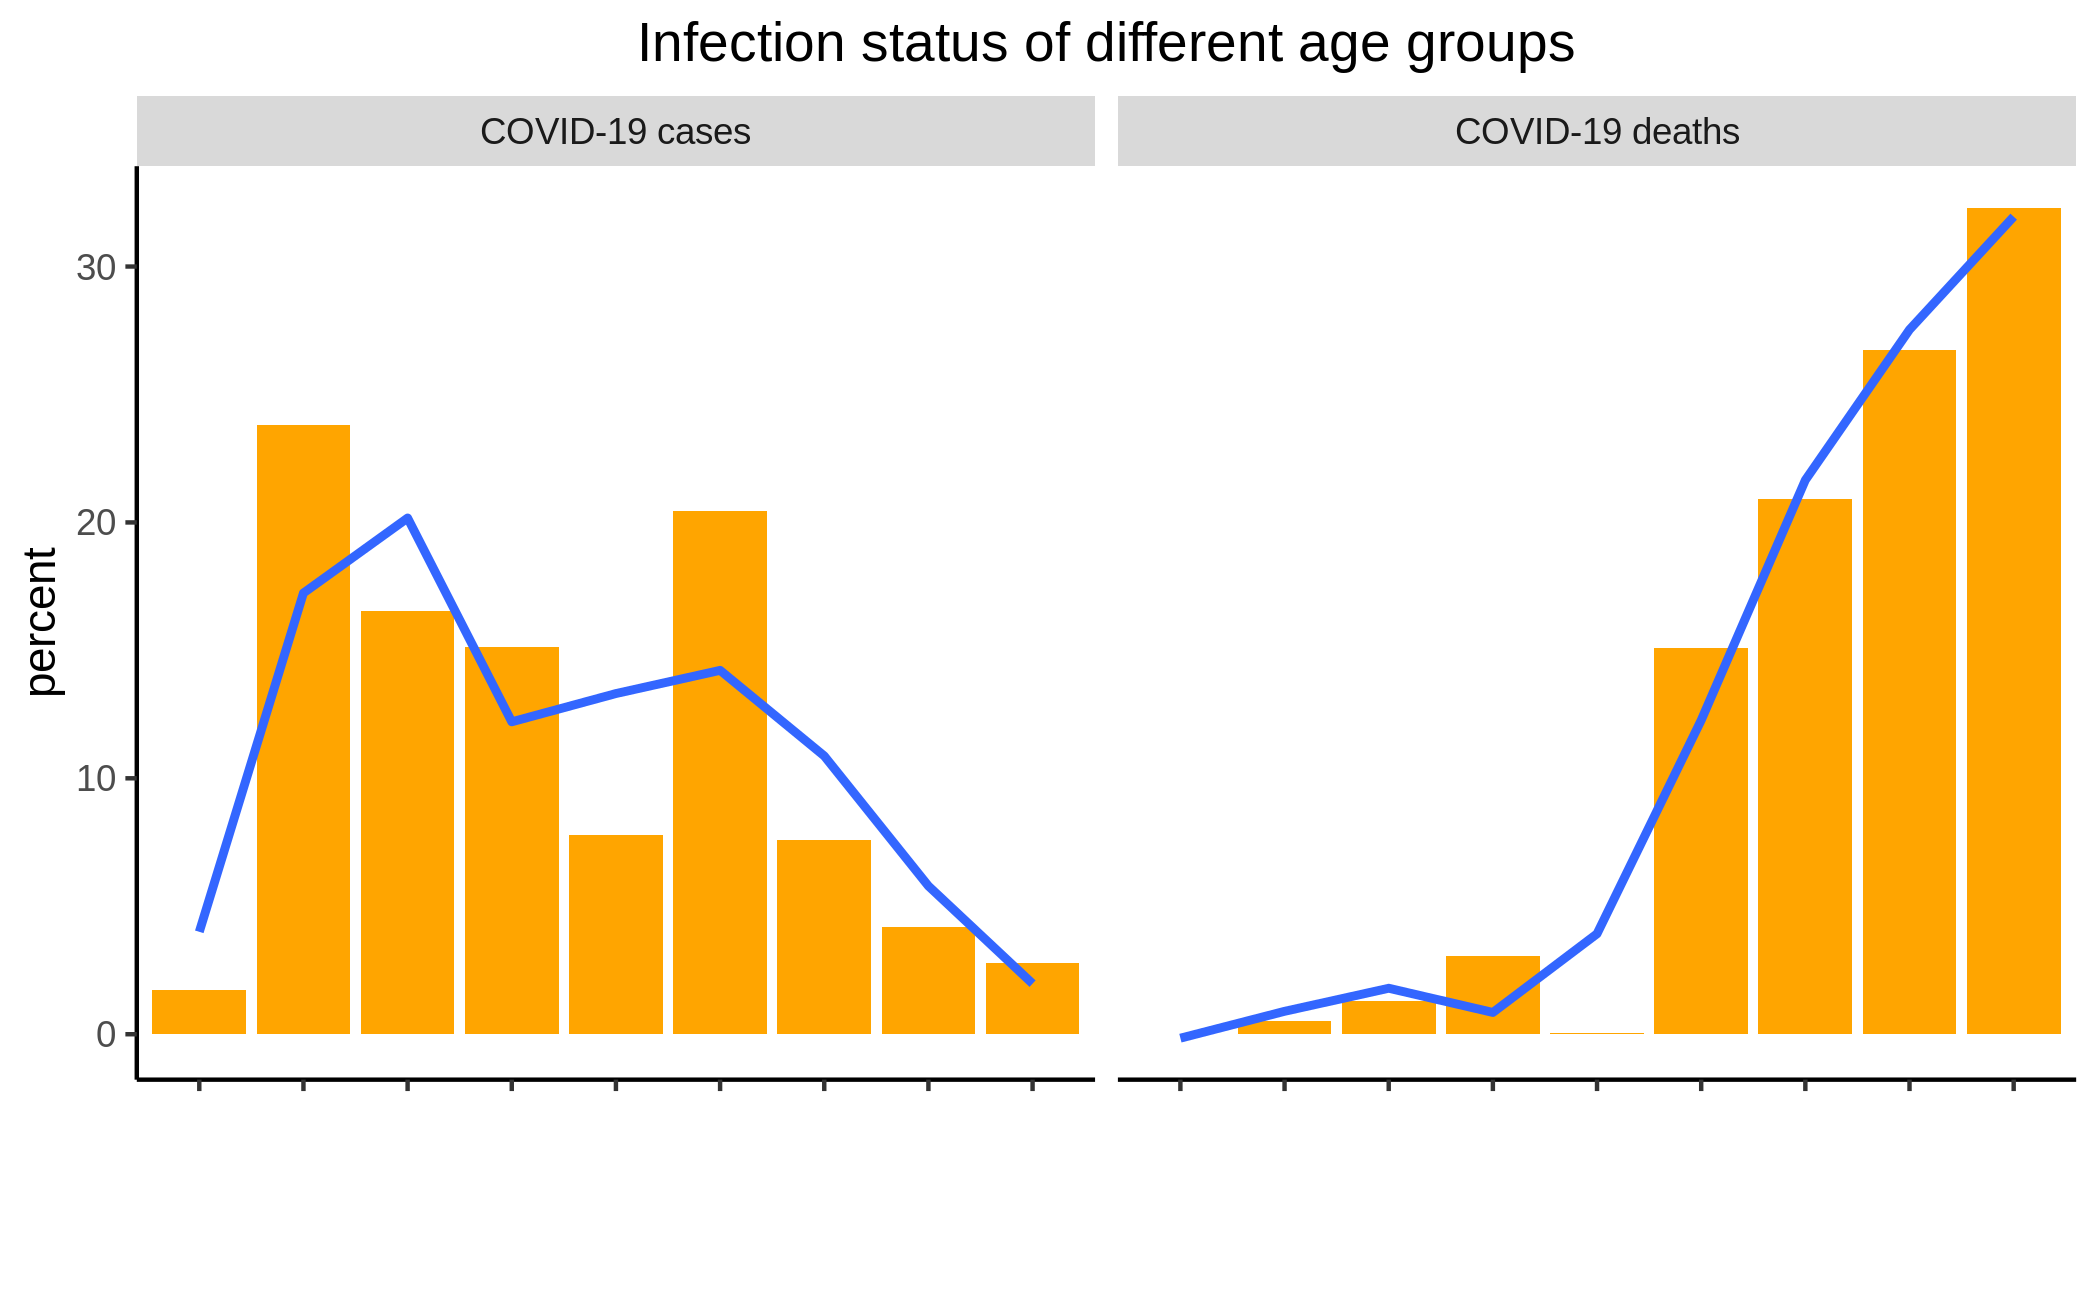
\includegraphics[width=1\linewidth]{age} \end{center}

This graph of infection of different age groups tells us the younger
people have a higher infection rate than other populations.
Nevertheless, the older people tends to be impacted seriously by the
virus, thus leading to the higher death rate among the population. We
add a smooth line to the differences using \texttt{loess} method.

\hypertarget{q4-population-infection-rate}{%
\subsubsection{Q4: Population Infection
Rate}\label{q4-population-infection-rate}}

The population infection rate in different states can serve as an
indicator of virus spreading level.

\begin{center}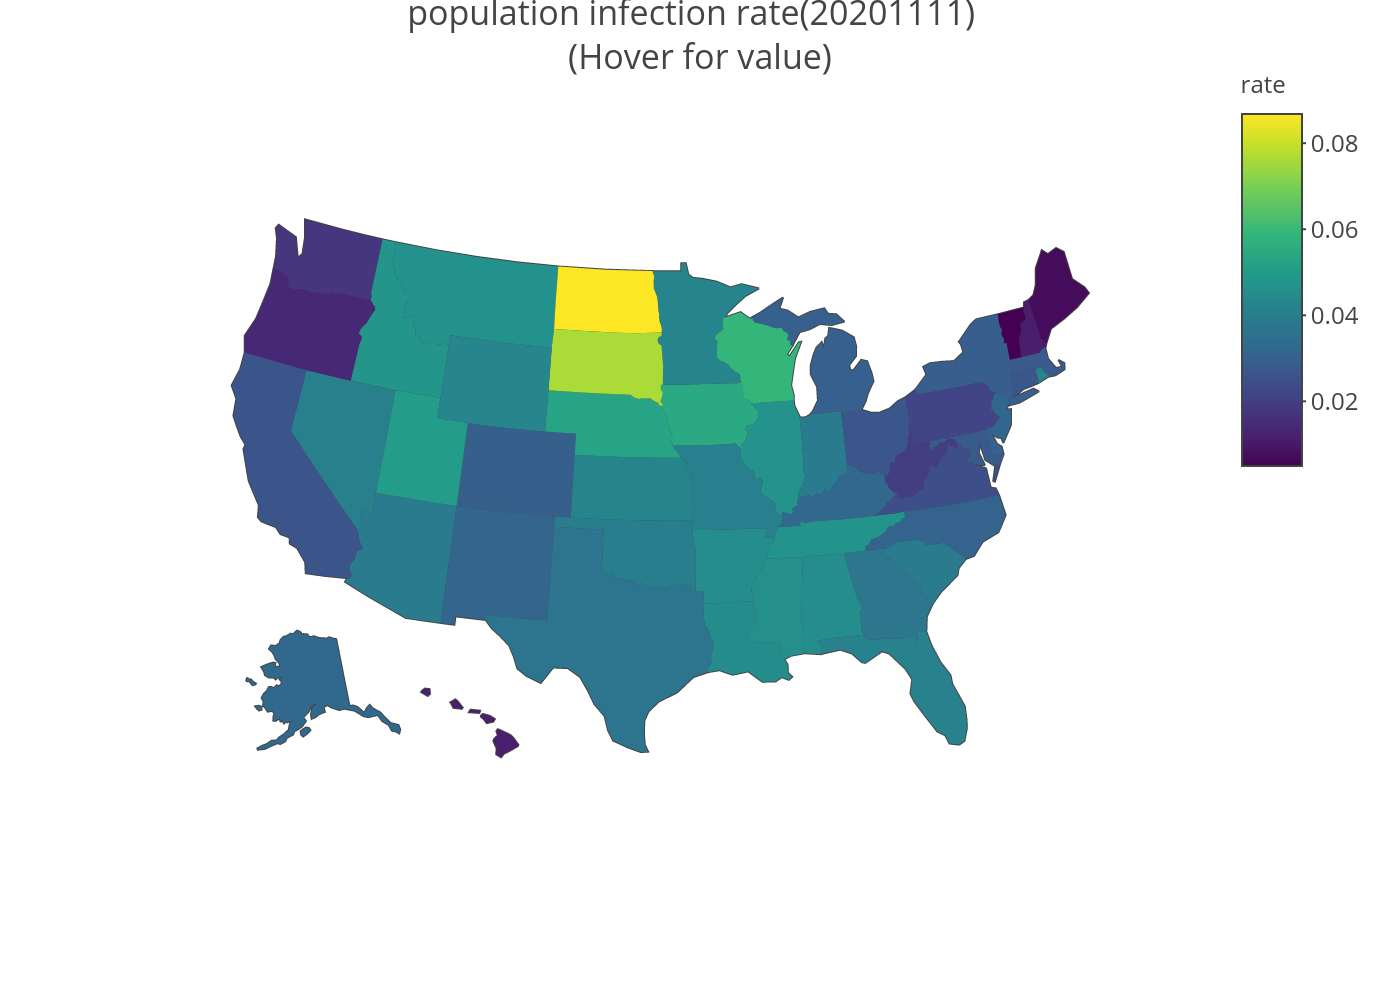
\includegraphics[width=1\linewidth]{infection_rate} \end{center}

From the map, we can see that different states have different population
infection rate now. Some states such as are serious than others. Another
thing to pay attention to is that the population infection rate has
reached a significant level of .

\hypertarget{q5-key-information}{%
\subsubsection{Q5: Key Information}\label{q5-key-information}}

The COVID Tracking Project also gathers notes from every state. These
notes are informative for us to know about what is happing with the
COVID-19 status with the state. In other words, we can catch the latest
and most important information reading these notes. Simple text-mining
like n-grams can give us a rough topic about the pandemic condition.
Here, we choose tri-grams.

\begin{center}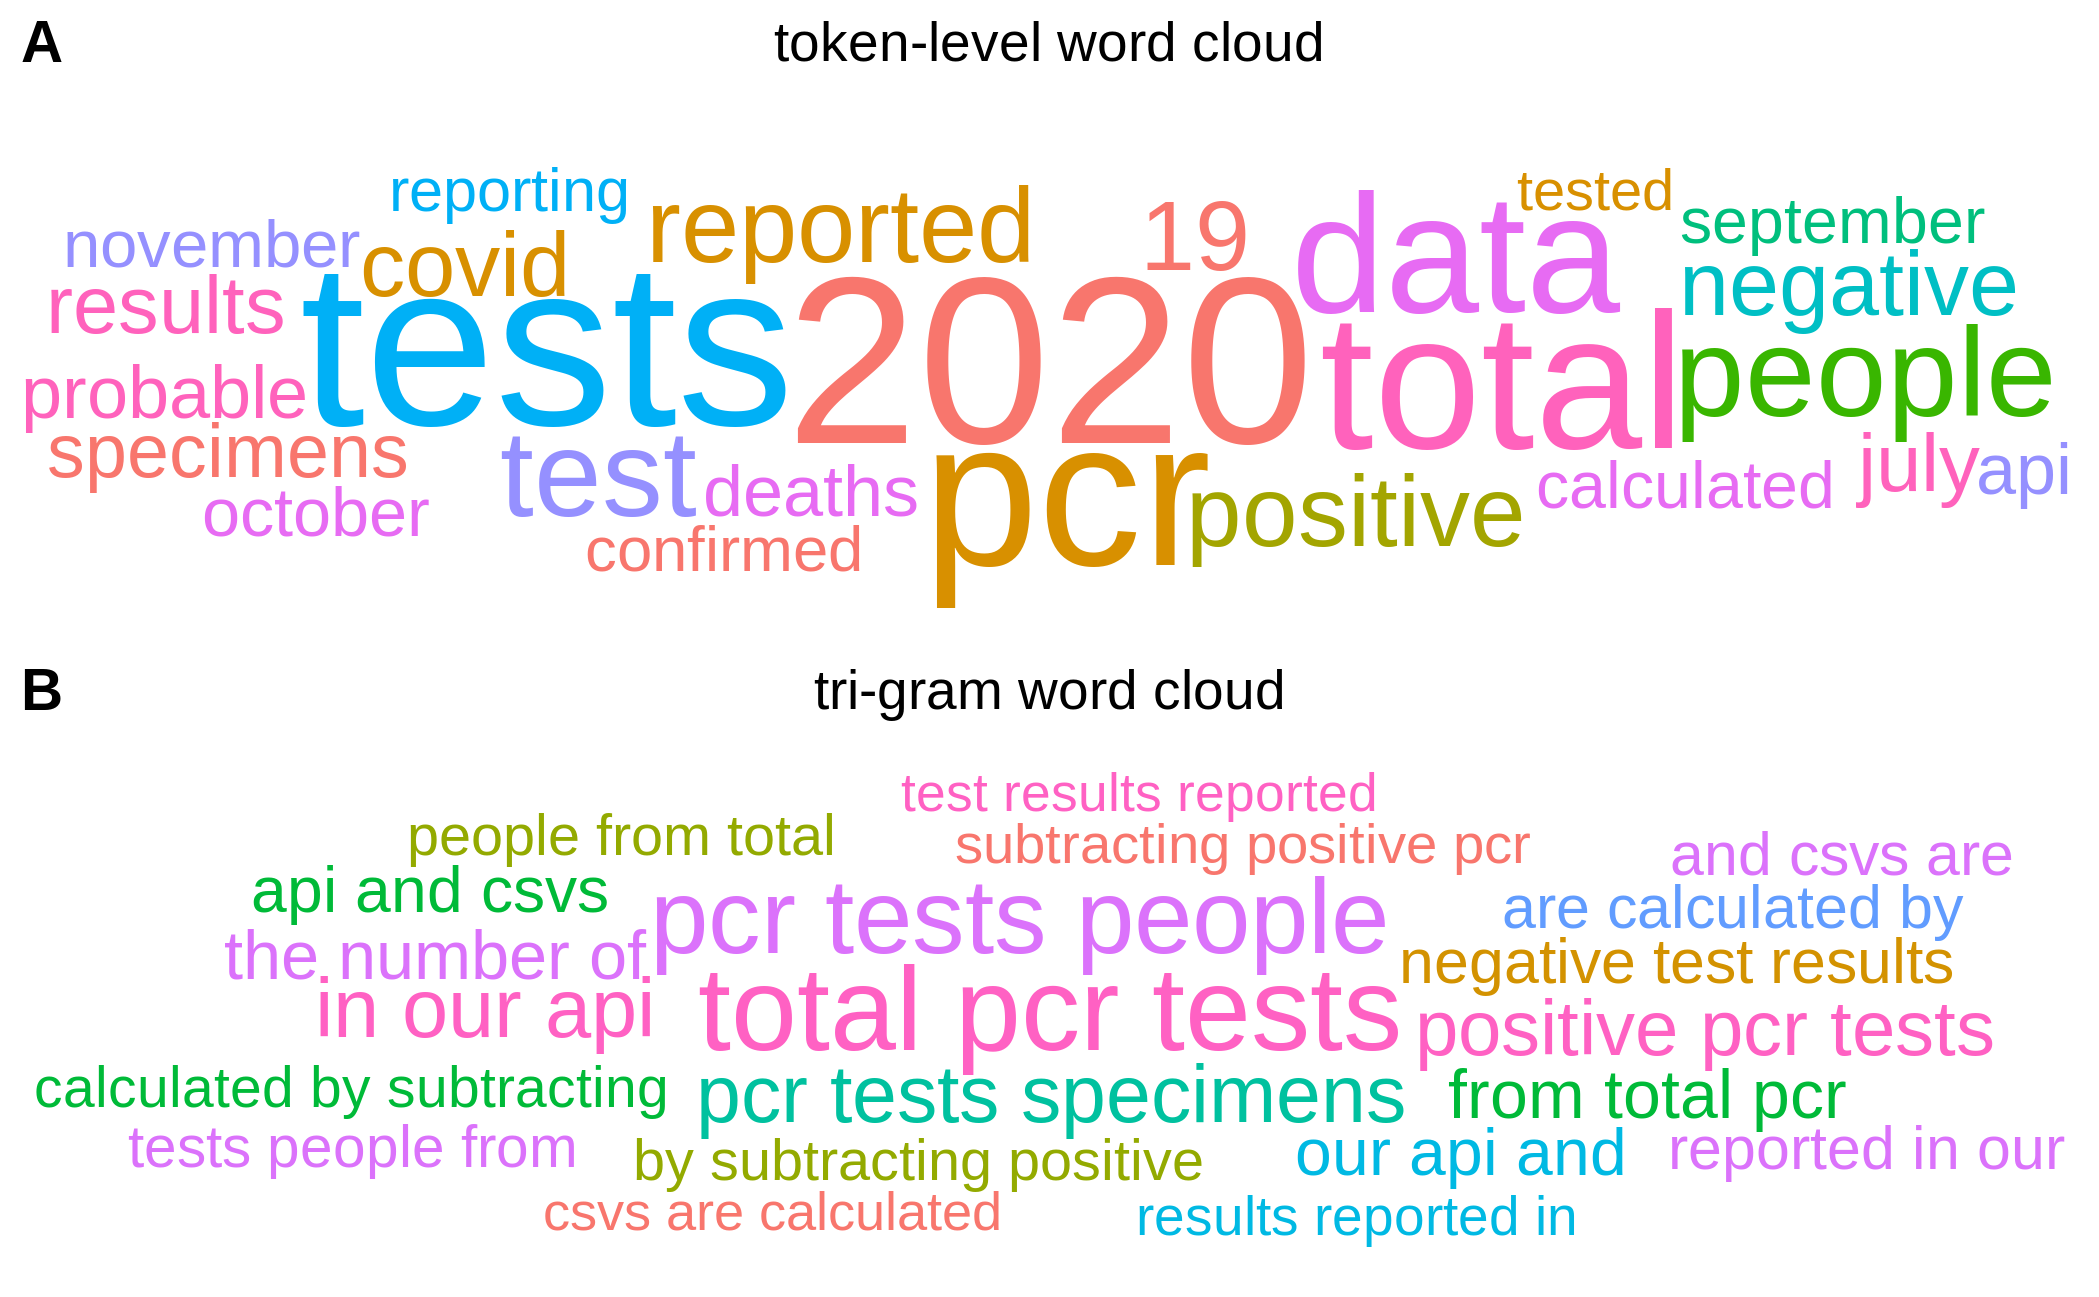
\includegraphics[width=1\linewidth]{wordcloud} \end{center}

From the statistics of tri-grams, we can infer that ``PCR test'' is the
most important information across all states. It means that most states
is mainly focusing on COVID-19 testing now.

\hypertarget{conclusion-and-summary}{%
\subsubsection{Conclusion and Summary}\label{conclusion-and-summary}}

How is the COVID-19 condition in the United States now?

To begin with, the COVID-19 condition is not optimistic now, we can see
the huge numbers of cases in the overview part. Firstly, the infection
is still continuously growing with a higher and higher growth rate.
Secondly, the virus infections and impacts are different in terms of
different age groups and races/ethnicities. Thirdly, The population
infection rate is different across different states and has already
reached a significant level of around 2\% now. Finally, most states are
mainly working on doing COVID-19 testing now, this is the key
information we should pay attention to.

\end{document}
